\documentclass[11pt,slidesonly,semrot,portrait,palatino]{book}
\usepackage{amssymb}
\usepackage{amsmath}
\usepackage{epsfig}

\newcommand{\simdot}{\stackrel{\cdot}{\sim}}
\newcommand{\bfbeta}{{\mbox{\boldmath$\beta$}}}
\newcommand{\bfep}{{\mbox{\boldmath$\epsilon$}}}
\newcommand{\bhat}{\hat{\beta}}
\newcommand{\btilde}{\tilde{\mbox{\boldmath$\beta$}}}
\newcommand{\bfmu}{{\mbox{\boldmath$\mu$}}}
\newcommand{\Var}{{\rm Var}}
\newcommand{\Cov}{{\rm Cov}}
\newcommand{\trt}{{\rm trt}}
\newcommand{\pr}{{\rm pr}}
\newcommand{\age}{{\rm age}}
\newcommand{\Sin}{\sum_{i=1}^N}
\newcommand{\Sjn}{\sum_{j=1}^N}
\newcommand{\ui}{{\bf u}_i}
\newcommand{\uj}{{\bf u}_j}
\newcommand{\bfx}{{\mbox{{\bf x}}}}
\newcommand{\bfp}{{\mbox{{\bf p}}}}
\newcommand{\hbfp}{\widehat{\mbox{{\bf p}}}}
\newcommand{\bfy}{{\mbox{{\bf y}}}}
\newcommand{\bfY}{{\mbox{{\bf Y}}}}
\newcommand{\bfZ}{{\mbox{{\bf Z}}}}
\newcommand{\bfa}{{\mbox{{\bf a}}}}
\newcommand{\bfb}{{\mbox{{\bf b}}}}
\newcommand{\bfg}{{\mbox{{\bf g}}}}
\newcommand{\bfU}{{\bf U}}
\newcommand{\bfu}{{\mbox{{\bf u}}}}
\newcommand{\bfz}{{\mbox{{\bf z}}}}
\newcommand{\logit}{{\mbox{{logit}}}}
\newcommand{\bfzero}{{\mbox{{\bf 0}}}}
\newcommand{\hbeta}{{\widehat \beta}}
\newcommand{\heta}{{\widehat \eta}}
\newcommand{\hsigma}{{\widehat \sigma}}
\newcommand{\hmu}{{\widehat \mu}}
\newcommand{\hpi}{{\widehat \pi}}
\newcommand{\cI}{{\cal I}}
\newcommand{\bsigma}{{\bar \sigma}}
\newcommand{\brho}{{\bar \rho}}
\newcommand{\bx}{ {\bar {x} } }
\newcommand{\bY}{ {\bar {Y} } }
\newcommand{\hY}{ {\widehat {Y} } }
\newcommand{\hp}{ {\widehat {p} } }
\newcommand{\hVar}{ {\widehat {Var} } }

%\setlength{\baselineskip}{2.5em}
\begin{document}
\setlength{\evensidemargin}{0in} \setlength{\oddsidemargin}{.5in}
\setlength{\topmargin}{0in} \setlength{\textwidth}{6in}
\setlength{\textheight}{9in} \setcounter{page}{29}
\setcounter{chapter}{2}
\chapter{Nonparametric methods to estimate survival}
\noindent

We will consider three methods for estimating a survivorship
function
$$S(t) = Pr(T \ge t)$$

without resorting to parametric methods:

\begin{itemize}
\item[(1)] {\bf Kaplan-Meier}
\item[(2)] {\bf Life-table} (Actuarial Estimator)
\item[(3)] {\bf Cumulative hazard estimator}
\end{itemize}
%%%%%%%%%%%%%%%%%%%%%%%%%%%%%%%%%%%%%%%%%%%%%%%%%%%%%%%%%%%5
\section{The Kaplan-Meier Estimator}

The Kaplan-Meier (or KM) estimator is probably the most
popular approach.  It can be justified from several
perspectives:

\begin{itemize}
\item product limit estimator
\item likelihood justification
\item redistribute to the right estimator
\end{itemize}
We will start with an intuitive motivation based on conditional
probabilities, then review some of the other justifications.
\newpage\noindent
\underline{\bf Motivation:}\\[1ex]
First, consider an example where there is no censoring. \\[1ex]
The following are times of remission (weeks) for 21 leukemia patients
receiving control treatment (Table 1.1 of Cox \& Oakes): \\[1.5ex]
\centerline{1, 1, 2, 2, 3, 4, 4, 5, 5, 8, 8, 8, 8, 11, 11, 12, 12, 15,
17, 22, 23}\\[2ex]
How would we estimate S(10), the probability that
an individual survives to time 10 or later?
\\[2ex]
What about $\tilde{S}(8)$?   Is it $\frac{12}{21}$ or $\frac{8}{21}$?\\[2ex]
Let's construct a table of $\tilde{S}(t)$:
%\vspace*{-1.5in}
\begin{center}
\begin{tabular}{cc}
Values of t   & ~~~~$\hat{S}(t)$~~~~ \\
\hline
$~~~~~ t \le 1 $  & 21/21=1.000 \\
$1 < t \le 2 $  & 19/21=0.905\\
$2 < t \le 3 $  & 17/21=0.809\\
$3 < t \le 4 $  & \\
$4 < t \le 5 $  & \\
$5 < t \le 8 $  & \\
$8 < t \le 11 $ &\\
$11 < t \le 12 $ &\\
$12 < t \le 15 $ &\\
$15 < t \le 17 $ &\\
$17 < t \le 22 $ &\\
$22 < t \le 23 $ &\\
\end{tabular}
\end{center}
%%%%%%%%%%%%%%%%%%%%%%%%%%%%%%%%%%%%%%%%%%%%%%%%%%%%%%%%%%%5
\subsection{Empirical Survival Function:}
When there is no censoring, the general formula is:
\begin{eqnarray*}
\tilde{S}(t) = \frac{\#~individuals~ with~T \ge t}
       {total~sample~size}
\end{eqnarray*}
\begin{figure}[h]
\centerline{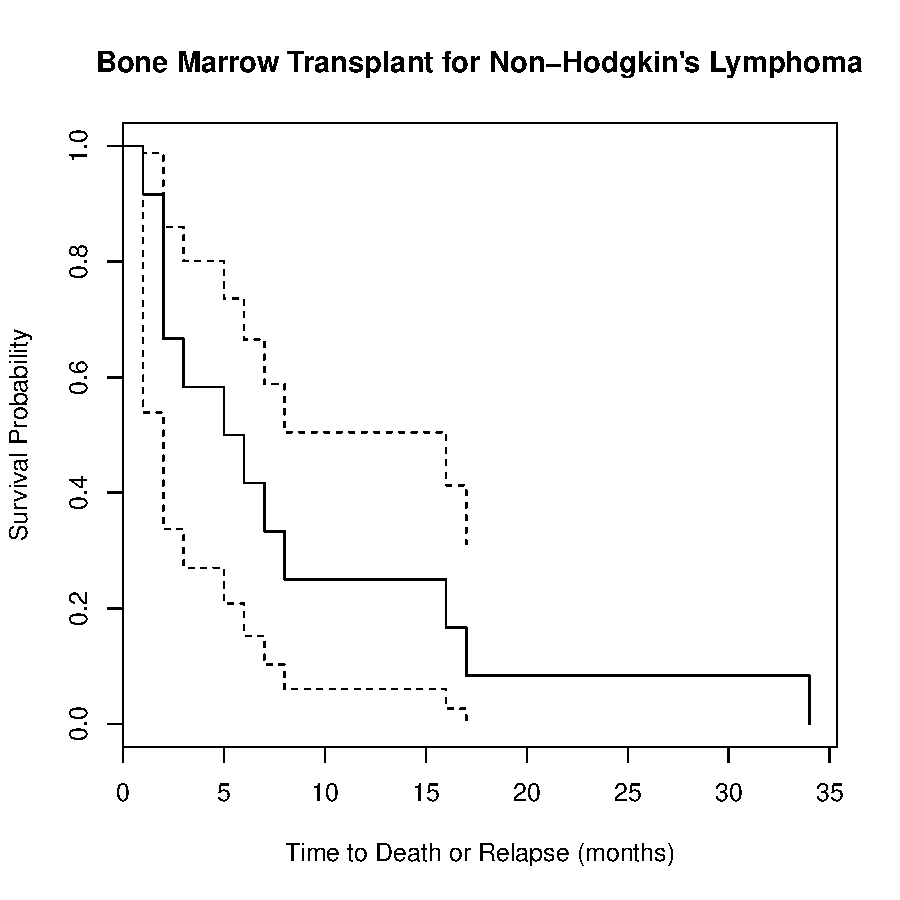
\includegraphics[width=3in]{surv_control.pdf}}
\caption{Example for leukemia data (control arm)}
\end{figure}
%%%%%%%%%%%%%%%%%%%%%%%%%%%%%%%%%%%%%%%%%%%%%%%%%%%%
\subsubsection{What if there is censoring?}

Consider the treated group from Table 1.1 of Cox and Oakes:\\
\[6^+,6,6,6,7,9^+,10^+,10,11^+,13,16,17^+\]
\[19^+,20^+,22,23,25^+,32^+,32^+,34^+,35^+\]


[Note: times with $^+$ are right censored]
\\
We know S(6)= 21/21, because everyone survived at least until time
6 or greater.  But, we can't say S(7) = 17/21, because we don't know
the status of the person who was censored at time 6.  \\[2ex]
\\
In a 1958 paper in the {\em Journal of the American Statistical
Association}, Kaplan and Meier
 proposed a way to nonparametrically estimate S(t),
even in the presence of censoring.  The method
is based on the ideas of {\bf conditional probability}.
%%%%%%%%%%%%%%%%%%%%%%%%%%%%%%%%%%%%%%%%%%%%%%%%%%%%
\subsection{A quick review of conditional probability:}

\subsubsection{Conditional Probability:} Suppose A and B are two events.
Then,
\[  P(A|B)  =    \frac { P(A \cap B)}  { P(B)}\]

\subsubsection{Multiplication law of probability}: can be obtained from
the above relationship, by multiplying both sides by $P(B)$:
\begin{eqnarray*}
P(A \cap B) & = & P(A|B) \, P(B)
\end{eqnarray*}

\subsection{Extension to more than 2 events:}
Suppose $A_1,  A_2 ...  A_k$ are k different events.  Then,
the probability of all k events happening together can be
written as a product of conditional probabilities:\\
\begin{eqnarray*}
   P(A_1 \cap A_2 ... \cap A_k)  & = &    P(A_k|A_{k-1} \cap ... \cap A_1) \times \\
         &  &   \times  P(A_{k-1}|A_{k-2} \cap ... \cap A_1) \\
         &  &     ...  \\
         &  &   \times P(A_2| A_1)\\
         &  &   \times P(A_1)\\
\end{eqnarray*}
%%%%%%%%%%%%%%%%%%%%%%%%%%%%%%%%%%%%%%%%%%%%%%%%%%%%
\subsubsection{Now, let's apply these ideas to estimate $S(t)$}
Suppose $a_k<t\le a_{k+1}$.  Then
\begin{eqnarray*}
S(t) & = & P(T \ge a_{k+1}) \\[1ex]
& = & P(T\ge a_1, T\ge a_2,\ldots,T\ge a_{k+1})\\[1ex]
& = & P(T\ge a_1) \times \prod_{j=1}^k \, P(T\ge a_{j+1}|T\ge a_j) \\[1ex]
& = &  \prod_{j=1}^k \, [1-P(T=a_j|T\ge a_j)]\\[1ex]
& = &  \prod_{j=1}^k \, [1-\lambda_j]
\end{eqnarray*}

So,
\begin{eqnarray*}
\hat{S}(t)
& \cong &  \prod_{j=1}^k \, \left(1-\frac{d_j}{r_j}\right) \\[1ex]
& = & \prod_{j:a_j<t}\left(1-\frac{d_j}{r_j}\right)
\end{eqnarray*}
where $d_j$ is the number of deaths at $a_j$ and $r_j$ is the number at risk at $a_j$
\subsection{Intuition behind the Kaplan-Meier Estimator}

Think of dividing the observed timespan of the study into
a series of fine intervals so that there is a separate
interval for each time of death or censoring:\\
\begin{center}
\begin{tabular}{l|p{.2in}|p{.2in}|p{.2in}
 |p{.2in}|p{.2in}|p{.2in}|p{.3in}|p{.2in}|p{.2in}|p{.2in}
 |p{.2in}|p{.2in}|p{.2in}}
  &   &  & D & & C & & C & D & D & D \\
  \hline
  \end{tabular}
  ~\\[2ex]
  \end{center}
Using the law of conditional probability,
 \begin{eqnarray*}
Pr(T \ge t) & = &
\prod_j Pr(\mbox{\small survive $j$-th interval $I_j$}~|
~\mbox{\small survived to start of $I_j$})
\end{eqnarray*}
where the product is taken over all the  intervals including or preceding time t.
\\[2ex]
\underline{There are possibilities for each interval:}
\begin{itemize}
     \item[(1)]  {\bf No events (death or censoring)} - conditional
     probability of surviving the interval is 1
     \item[(2)]  {\bf Censoring} - assume they survive to the
     end of the interval, so that the conditional
     probability of surviving the interval is 1
     \item[(3)]  {\bf Death, but no censoring}  - conditional
     probability of {\em not} surviving the interval is \# deaths (d)
     divided by \# `at risk' (r) at the beginning of the
     interval. So the conditional probability of surviving the
     interval is $1-(d/r)$.
     \item[(4)]  {\bf Tied deaths and censoring} -
         assume censorings last
     to the end of the interval, so that conditional
     probability of surviving the interval is still $1-(d/r)$
     \end{itemize}
\underline{\bf General Formula for $j$th interval:}\\[1ex]
It turns out we can write a general formula for the
conditional probability of surviving the $j$-th interval
that holds for all 4 cases:
$$1 - \frac{d_j}{r_j}$$
We could use the same approach by grouping the event times into
intervals (say, one interval for each month), and then counting
up the number of deaths (events) in each to estimate the probability
of surviving the interval (this is called the {\em lifetable estimate}).
\\[2ex]
However, the assumption that those censored last until the end
of the interval wouldn't be quite accurate, so we would end
up with a cruder approximation.
\\[2ex]
As the intervals get finer and finer, the approximations made in
estimating the probabilities of getting through each interval
become smaller and smaller, so that the estimator
converges to the true $S(t)$.
\\[2ex]
This intuition clarifies why an alternative name for the KM is
the {\bf product limit estimator}.
%%%%%%%%%%%%%%%%%%%%%%%%%%%%%%%%%%%%%%%%%%%%%%%%%%%%

\begin{center}
\fbox{\begin{tabular}{ccc}
\multicolumn{3}{c}{\bf The Kaplan-Meier estimator of the survivorship }\\
\multicolumn{3}{c}{\bf function (or survival probability) $S(t)=Pr(T \ge  t)$ is:}\\[2ex]
\multicolumn{3}{c}{ $\hat{S}(t)$ =
{ $\prod_{j: \tau_j < t} \frac{ r_j - d_j } {r_j}$} =   { $\prod_{j: \tau_j < t} \left (1 - \frac{d_j}{r_j}\right)$}}
\end{tabular}}
\end{center}
where,
\small
\begin{itemize}
\item   $\tau_1,... \tau_K$ are the $K$ distinct death times
observed in the sample
\item  $d_j$ is the number of deaths at $\tau_j$
\item  $r_j$ is the number of individuals ``at risk'' right before the $j$-th
death time (everyone dead or censored \underline{at or after} that
time).
\item   $c_j$ is the number of censored observations between the
$j$-th and $(j+1)$-st death times.  Censorings tied
at $\tau_j$ are included in $c_j$
   \end{itemize}
\normalsize
{\bf Note:  two useful formulas are:}
\begin{eqnarray*}
(1)~~~ r_j & = & r_{j-1} - d_{j-1} - c_{j-1}\\[1ex]
(2)~~~ r_j & = & \sum_{l \ge j} (c_l+d_l)
\end{eqnarray*}
%%%%%%%%%%%%%%%%%%%%%%%%%%%%%%%%%%%%%%%%%%%%%%%%%%%%


\subsection{Calculating the KM - Cox and Oakes example}
Make  a table with a row for every  death or censoring time:
\begin{center}
\begin{tabular}{ccccccc}
$\tau_j$ & ~~$d_j$~~   & $~~c_j~~$  & $~~r_j~~$ & ~~~$1-(d_j/r_j)$~~~
& $\hat{S}(\tau_j^+ )$ \\  \hline
6  &  3     &  1      &  21     & $\frac{18}{21}$ = 0.857 \\
7  &  1     &  0      &  17     & \\
9  &  0     &  1      &  16     & \\
10 \\
11 \\
13 \\
16 \\
17 \\
19 \\
20 \\
22 \\
23 \\
\end{tabular}
\end{center}
{\bf Note that:}
 \begin{itemize}
 \item $\hat{S}(t^+)$ only changes at death (failure) times
 \item $\hat{S}(t^+)$ is 1 up to the first death time
 \item $\hat{S}(t^+)$ only goes to 0 if the last event is a death
 \end{itemize}
%%%%%%%%%%%%%%%%%%%%%%%%%%%%%%%%%%%%%%%%%%%%%%%%%%%%
\normalsize

\begin{figure}[h]
\centerline{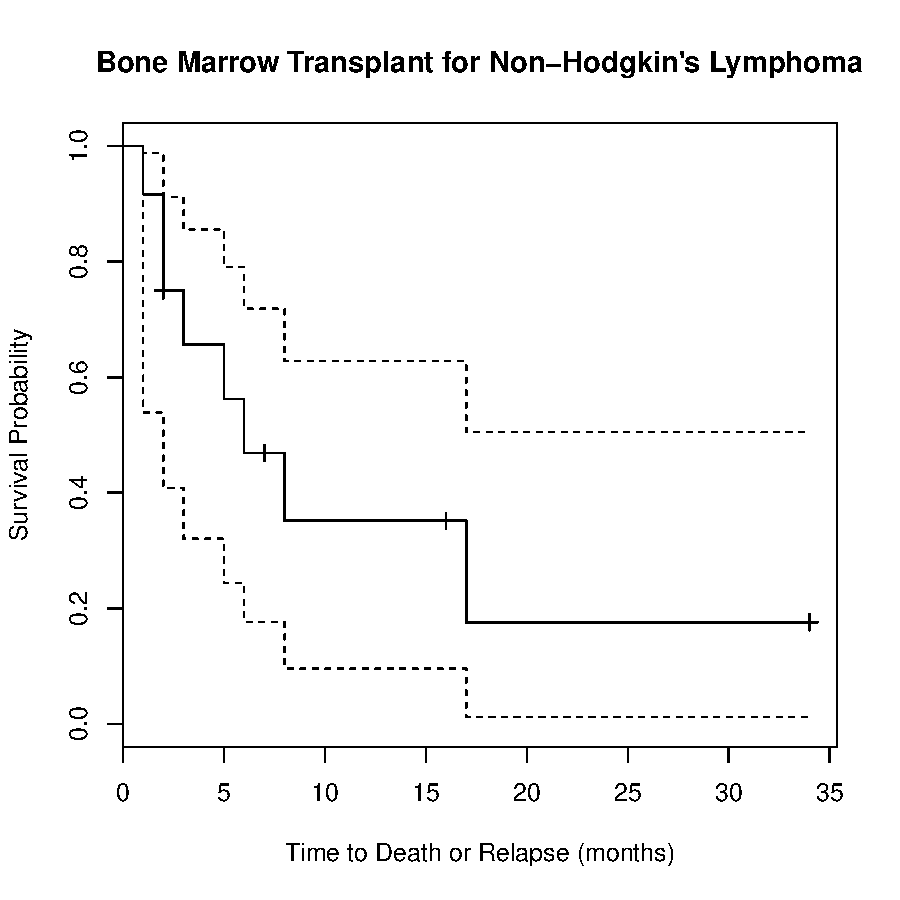
\includegraphics[width=3in]{surv_trt.pdf}}
\caption{KM plot for treated leukemia patients}
\end{figure}
\noindent
{\bf Note: most statistical software packages summarize
the KM survival function at $\tau_j^{+}$, i.e.,
{\em just after} the time of the $j$-th failure.}
\\[2ex]
{ \bf In other words, they provide $\hat{S}(\tau_j^+)$}.
\\[2ex]
When there is no censoring, the empirical survival estimate
would then be:
\begin{eqnarray*}
\tilde{S}(t^+) = \frac{\#~individuals~ with~T > t}{total~sample~size}
\end{eqnarray*}
%%%%%%%%%%%%%%%%%%%%%%%%%%%%%%%%%%%%%%%
\newpage
\subsubsection{Output from STATA KM Estimator:}
\small
\begin{verbatim}
    failure time:  weeks
  failure/censor:  remiss

           Beg.          Net   Survivor     Std.
  Time    Total   Fail   Lost  Function    Error   [95% Conf. Int.]
-------------------------------------------------------------------
     6       21      3      1    0.8571   0.0764   0.6197  0.9516
     7       17      1      0    0.8067   0.0869   0.5631  0.9228
     9       16      0      1    0.8067   0.0869   0.5631  0.9228
    10       15      1      1    0.7529   0.0963   0.5032  0.8894
    11       13      0      1    0.7529   0.0963   0.5032  0.8894
    13       12      1      0    0.6902   0.1068   0.4316  0.8491
    16       11      1      0    0.6275   0.1141   0.3675  0.8049
    17       10      0      1    0.6275   0.1141   0.3675  0.8049
    19        9      0      1    0.6275   0.1141   0.3675  0.8049
    20        8      0      1    0.6275   0.1141   0.3675  0.8049
    22        7      1      0    0.5378   0.1282   0.2678  0.7468
    23        6      1      0    0.4482   0.1346   0.1881  0.6801
    25        5      0      1    0.4482   0.1346   0.1881  0.6801
    32        4      0      2    0.4482   0.1346   0.1881  0.6801
    34        2      0      1    0.4482   0.1346   0.1881  0.6801
    35        1      0      1    0.4482   0.1346   0.1881  0.6801
\end{verbatim}
\normalsize
%%%%%%%%%%%%%%%%%%%%%%%%%%%%%%%%%%%%%%%%%%%%%%%%%%%%
\newpage
\subsection{Two Other Justifications for KM Estimator}

\subsubsection{I. Likelihood-based derivation (Cox and Oakes)}

For a discrete failure time variable, define:
\begin{center}
\begin{tabular}{ll}
$d_j$ &  number of failures at $a_j$\\
$r_j$ &  number of individuals at risk at $a_j$ \\
      & (including those  censored at $a_j$).\\
$\lambda_j$ & Pr(death) in $j$-th interval \\
            & (conditional on survival to start of interval)\\
\end{tabular}
\end{center}

The likelihood is that of $g$ independent binomials:
\begin{eqnarray*}
L(\bf \lambda) & = & \prod_{j=1}^g
\lambda_j^{d_j}(1-\lambda_j)^{r_j-d_j}
\end{eqnarray*}

Therefore, the {\bf maximum likelihood estimator} of
$\lambda_j$ is:
 \[\hat{\lambda}_j=d_j/r_j\]

Now we plug in the MLE's of $\lambda$ to estimate S(t)::
\begin{eqnarray*}
\hat{S}(t) & = & \prod_{j:a_j<t}(1-\hat{\lambda}_j)\\[2ex]
 & = & \prod_{j:a_j<t}\left(1-\frac{d_j}{r_j}\right)
\end{eqnarray*}
%%%%%%%%%%%%%%%%%%%%%%%%%%%%%%%%%%%%%%%%%%%%%%%%%%%%
\subsubsection{II. Redistribute to the right justification (Efron, 1967)}

In the absence of censoring, $\hat{S}(t)$ is just the proportion of
individuals with $T\ge t$.  The idea behind Efron's approach
is to spread the contributions of censored observations out over all the
possible times to their right.
\\[2ex]
\underline{\bf Algorithm:}
\begin{itemize}
\item Step (1):  arrange the n observed times (deaths or censorings) in
increasing order.
If there are ties, put censored after deaths.
\item Step (2):  Assign weight $(1/n)$ to each time.
\item Step (3):  Moving from left to right, each time you encounter
a censored observation, distribute its mass to all times to its right.
\item Step (4): Calculate $\hat{S}_j$ by subtracting the final weight
 for time $j$ from $\hat{S}_{j-1}$
\end{itemize}
%%%%%%%%%%%%%%%%%%%%%%%%%%%%%%%%%%%%%%%%%%%%%%%%%%%%
\subsubsection{Example of ``redistribute to the right'' algorithm}
Consider the following event times:
\begin{center}
2,~ 2.5$+$,~ 3,~ 3,~ 4,~ 4.5$+$,~ 5,~ 6,~ 7
\end{center}
The algorithm goes as follows:
\begin{center}
   \begin{tabular}{ccccc}\\
(Step 1) & & & & (Step 4)\\
       Times  & ~Step 2~ & ~Step 3a~ & ~Step 3b~ & $\hat{S}(\tau_j)$ \\\hline
       2 & 1/9=0.11  & & & 0.889\\
       2.5$^+$ & 1/9=0.11 & 0 & & 0.889\\
       3 & 2/9=0.22 & 0.25 & & 0.635\\
       4 & 1/9=0.11 & 0.13 & & 0.508\\
       4.5$^+$ & 1/9=0.11 & 0.13 & 0 & 0.508\\
       5 & 1/9=0.11 & 0.13 & 0.17 & 0.339\\
       6 & 1/9=0.11 & 0.13 & 0.17 & 0.169\\
       7 & 1/9=0.11 & 0.13 & 0.17 & 0.000\\ \hline
       \end{tabular}
\end{center}
This comes out the same as the product limit approach.
%%%%%%%%%%%%%%%%%%%%%%%%%%%%%%%%%%%%%%%%%%%%%%%%%%%%
\subsection{Properties of the KM estimator}
\subsubsection{In the case of no censoring:}
\begin{eqnarray*}
\hat{S}(t) = \tilde{S}(t) = \frac{\#~deaths~at~ t~ or~ greater}{n}
\end{eqnarray*}
\vspace*{.2in}
where n is the number of individuals in the study.

This is just like an estimated probability from
a binomial distribution, so we have:
\[  \hat{S}(t) \simeq ~{\cal N}\left(S(t),~S(t)[1-S(t)]/n\right)   \]
{\bf How does censoring affect this?}
    \begin{itemize}
\item  $\hat{S}(t)$ is still approximately normal
\item  The mean of $\hat{S}(t)$ converges to the true S(t)
\item  The variance is a bit more complicated (since the denominator
$n$ includes some censored observations).
\end{itemize}
Once we get the variance, then we can construct (pointwise)
$(1-\alpha)$\% confidence
bands about $\hat{S}(t)$:
\[   \hat{S}(t)  \pm z_{1-\alpha/2} \, se[\hat{S}(t)] \]
%%%%%%%%%%%%%%%%%

\subsection{Greenwood's formula}
{\bf (Collett 2.1.3)} We can think of the KM estimator as
\[  \hat{S}(t) = \prod_{j: \tau_j < t} (1-\hat{\lambda}_j) \]
where $\hat{\lambda}_j = d_j / r_j.$
Since the $\hat\lambda_j$'s are just binomial proportions, we can
apply standard likelihood theory to show that each $\hat{\lambda}_j$ is
approximately normal, with mean the true $\lambda_j$, and
\begin{eqnarray*}
var(\hat    {\lambda}_j) & \approx &
\frac{\hat{\lambda}_j (1-\hat{\lambda}_j)}{r_j}
\end{eqnarray*}
The $\hat{\lambda}_j$'s are independent in large samples.
Since $\hat{S}(t)$ is a function of the $\lambda_j$'s, we
can estimate its variance using the {\bf delta method}:
\begin{quote}
If $Y$ is normal with mean $\mu$ and variance $\sigma^2$,
then $g(Y)$ is approximately normally distributed with
mean $g(\mu)$ and variance $[g'(\mu)]^2 \sigma^2$.
\end{quote}
%%%%%%%%%%%%%%%%%%%%%%%%%%%%%%%%%%%%%%%%%%%%%%%%%%%%


\subsubsection{Two specific examples of the delta method:}
\begin{itemize}
\item[(A)] $Z = log(Y)$
\begin{eqnarray*}
\mbox{then}~~~
Z \sim N\left[log(\mu),\left(\frac{1}{\mu}\right)^2 \sigma^2\right]
\end{eqnarray*}

\item[(B)] $Z = exp(Y)$
\begin{eqnarray*}
\mbox{then}~~~
Z \sim N\left[e^{\mu}, [e^{\mu}]^2 \sigma^2\right]
\end{eqnarray*}
\end{itemize}
The examples above use the following results from calculus:
\begin{eqnarray*}
\frac{d}{dx} \, \log u &=& \frac{1}{u} \; \left(\frac{du}{dx}\right)\\[2ex]
\frac{d}{dx} \, e^u &=& e^u  \; \left(\frac{du}{dx}\right)
\end{eqnarray*}
%%%%%%%%%%%%%%%%%%%%%%%%%%%%%%%%%%%%%%%%%%%%%%%%%%%%
Instead of dealing with $\hat{S}(t)$ directly, we will look at its
log:\\
\[ \log[\hat{S}(t)] = \sum_{j: \tau_j < t} \log(1-\hat{\lambda}_j)  \]
Thus, by approximate independence of the $\hat{\lambda}_j$'s,
\begin{eqnarray*}
var(\log[\hat{S}(t)]) &=& \sum_{j: \tau_j < t} var[\log(1-\hat{\lambda}_j)]\\
\end{eqnarray*}
By (A)
\begin{eqnarray*}
var(\log[\hat{S}(t)]) & = & \sum_{j: \tau_j < t} \left( \frac{1}{1-\hat{\lambda}_j} \right)^2
 var(\hat{\lambda}_j) \\
 &=& \sum_{j: \tau_j < t} \left(\frac{1}{1-\hat{\lambda}_j}\right)^2
 \hat{\lambda}_j (1-\hat{\lambda}_j)/r_j \\
 &=& \sum_{j: \tau_j < t} \frac{\hat{\lambda}_j}{(1-\hat{\lambda}_j) r_j} = \sum_{j: \tau_j < t} \frac{d_j}{(r_j-d_j) r_j}
 \end{eqnarray*}
Since $\hat{S}(t) = \exp[\log[\hat{S}(t)]]$, (by B),
\begin{eqnarray*}
var(\hat{S}(t)) & = & [\hat{S}(t)]^2 var\left[\log[\hat{S}(t)]\right]
\end{eqnarray*}
\begin{center}
\fbox{\begin{tabular}{c}
\multicolumn{1}{l}{\bf Greenwood's Formula:}\\[1ex]
\multicolumn{1}{r}{~~~~~~~~~~$var(\hat{S}(t)) =  [\hat{S}(t)]^2
\sum_{j: \tau_j < t} \frac{d_j}{(r_j-d_j) r_j}$}
\end{tabular}}\end{center}
%%%%%%%%%%%%%%%%%%%%%%%%%%%%%%%%%%%%%%%%%%%%%%%%%%%
\subsection{Confidence intervals}

For a 95\% confidence interval, we could use
\[   \hat{S}(t)  \pm z_{1-\alpha/2} \, se[\hat{S}(t)] \]
where $se[\hat{S}(t)]$ is calculated using Greenwood's formula.
\\[2ex]
{\bf Problem:}  This approach can yield values $>1$ or $<0$.
\\[2ex]
{\bf Better approach:}  Get a 95\% confidence interval for
$$L(t) = \log(-\log(S(t)))$$
Since this quantity is unrestricted, the confidence interval will
be in the right range when we transform back.
\\[2ex]
{\bf To see why this works, note the following:}
\begin{itemize}
\item Since $\hat{S}(t)$ is an estimated probability
$$0 \leq \hat{S}(t) \leq 1$$
\item Taking the log of $\hat{S}(t)$ and bounds:
$$- \infty \le \log[\hat{S}(t)] \leq 0$$
\item Taking the opposite:
$$ 0 \le -\log[\hat{S}(t)] \leq \infty$$
\item Taking the log again:
$$ - \infty \le \log\left[-\log[\hat{S}(t)]\right] \leq \infty$$
\end{itemize}
To transform back, reverse steps with $S(t)=\exp(-\exp(L(t))$
%%%%%%%%%%%%%%%%%%%%%%%%%%%%%%%%%%%%%%%%%%%%%%%%%%%
\subsubsection{Log-log Approach for Confidence Intervals:}
\begin{itemize}
\item[(1)] Define $L(t) = \log(-\log(S(t)))$
\item[(2)] Form a 95\% confidence interval for $L(t)$ based on
$\hat{L}(t)$, yielding $[\hat{L}(t)-A,\hat{L}(t)+A]$
\item[(3)] Since $S(t)=\exp(-\exp(L(t))$, the confidence bounds
for the 95\% CI on $S(t)$ are:
$$[exp(-e^{(\hat{L}(t)+A)}),exp(-e^{(\hat{L}(t)-A)})]$$
(note that the upper and lower bounds switch)
\item[(4)] Substituting $\hat{L}(t)=\log(-\log(\hat{S}(t)))$
back into the above bounds, we get confidence bounds of
$$([\hat{S}(t)]^{e^A},[\hat{S}(t)]^{e^{-A}})$$
\end{itemize}
%%%%%%%%%%%%%%%%%%%%%%%%%%%%%%%%%%%%%%%%%%%%%%%%%%%

{\bf What is A?}
\begin{itemize}
\item $A$ is $1.96 \, se(\hat{L}(t))$
\item To calculate this, we need to calculate
\begin{eqnarray*}
var(\hat{L}(t)) & = & var\left[\log(-\log(\hat{S}(t)))\right]
\end{eqnarray*}
\item From our previous calculations, we know
\begin{eqnarray*}
var(\log[\hat{S}(t)]) & = &
     \sum_{j: \tau_j < t} \frac{d_j}{(r_j-d_j) r_j}
\end{eqnarray*}

\item Applying the delta method as in example (A), we get:
\begin{eqnarray*}
var(\hat{L}(t))& = & var(\log(-\log[\hat{S}(t)])) \\ & = &
\frac{1}{[\log \,\hat{S}(t)]^2} \sum_{j: \tau_j < t} \frac{d_j}{(r_j-d_j) r_j}
\end{eqnarray*}
\item We take the square root of the above to get $se(\hat{L}(t))$,
and then form the confidence intervals as:
$$\hat{S}(t)^{e^{\pm 1.96 \, se(\hat{L}(t)) }}$$
\item This is the approach that Stata uses.  R also
gives an option to calculate these bounds.
\end{itemize}
%%%%%%%%%%%%%%%%%%%%%%%%%%%%%%%%%%%%%%%%%%%%%%%%%%%

\subsection{Summary of Confidence Intervals on $S(t)$}
\begin{itemize}
\item Calculate $\hat{S}(t) \pm 1.96 \, se[\hat{S}(t)]$
where $se[\hat{S}(t)]$ is calculated using Greenwood's formula,
and replace negative lower bounds by 0 and upper bounds greater than 1
by 1 (not very satisfactory).
\begin{itemize}
\item Recommended by Collett
\item This is the default using SAS
\end{itemize}
\item Use a log transformation to stabilize the variance and allow for
non-symmetric confidence intervals.  This is what is normally done for
the confidence interval of an estimated odds ratio.
\begin{itemize}
\item Use $var[\log(\hat{S}(t))] =
\sum_{j: \tau_j < t} \frac{d_j}{(r_j-d_j) r_j}$
already calculated as part of Greenwood's formula
\item This is the default in R
\end{itemize}
\item Use the log-log transformation just described
\begin{itemize}
\item Somewhat complicated, but always yields proper bounds
\item This is the default in Stata!
\end{itemize}
\end{itemize}
%%%%%%%%%%%%%%%%%%%%%%%%%%%%%%%%%%%%%%%%%%%%%%%%%%%%
\normalsize


\subsection{Software for Kaplan-Meier Curves}
\begin{itemize}
\item  Stata - stset and sts commands
\item  SAS  - {\sc proc lifetest}
\item  R - surv.fit(time,censor)
\end{itemize}
\subsubsection{Defaults for Confidence Interval Calculations}
\begin{itemize}
\item Stata - ``log-log'' $\Rightarrow \hat{L}(t) \pm 1.96 \,
se[\hat{L}(t)]$ \\
where $L(t) = \log[-\log(S(t))]$
\item SAS - ``plain'' $\Rightarrow \hat{S}(t) \pm 1.96\,
se[\hat{S}(t)]$
\item R - ``log'' $\Rightarrow \log{S}(t) \pm 1.96 \,
se[\log(\hat{S}(t))]$\\
but R will also give either of the other two options
if you request them.
\end{itemize}
%%%%%%%%%%%%%%%%%%%%%%%%%%%%%%%%%%%%%%%
\subsubsection{R Output for Treated Leukemia Patients:}
\begin{verbatim}
 time n.risk n.event survival std.err lower 95% CI upper 95% CI
    1     12       1    0.917  0.0798       0.5390        0.988
    2     11       2    0.750  0.1250       0.4084        0.912
    3      8       1    0.656  0.1402       0.3204        0.856
    5      7       1    0.562  0.1482       0.2437        0.791
    6      6       1    0.469  0.1503       0.1762        0.718
    7      5       0    0.469  0.1503       0.1762        0.718
    8      4       1    0.352  0.1517       0.0956        0.628
   16      3       0    0.352  0.1517       0.0956        0.628
   17      2       1    0.176  0.1456       0.0120        0.505
   34      1       0    0.176  0.1456       0.0120        0.505
\end{verbatim}
%%%%%%%%%%%%%%%%%%%%%%%%%%%%%%%%%%%%%%%

\normalsize
\newpage

%\begin{figure}[h]
%\centerline{\includegraphics[width=3in]{leukem_splus.pdf}}
%\caption{\label{KMsurvCI}KM Survival Estimate and Confidence intervals}
%\end{figure}
%%%%%%%%%%%%%%%%%%%%%%%%%%%%%%%%%%%%%%%

\subsection{Means, Medians, Quantiles based on the KM}
\begin{itemize}
\item  {\bf Mean:}  $\sum_{j=1}^{k} \tau_j \, Pr(T=\tau_j)$
\item  {\bf Median} - by definition, this is the time, $\tau$,
such that $S(\tau)=0.5$.  However, in practice, it is defined as
the smallest time such that $\hat{S}(\tau)\leq 0.5$.
The median is more appropriate for censored survival data
than the mean.

For the treated leukemia patients, we find:
\begin{eqnarray*}
\hat{S}(22) = 0.5378 ~~~~~~~ \hat{S}(23) = 0.4482
\end{eqnarray*}
The median is thus 23.   This can also be seen visually
in Figure~\ref{KMsurvCI}    .
\item  {\bf Lower quartile (25$^{th}$ percentile):}\\
the smallest time (LQ) such that $\hat{S}(LQ)\leq 0.75$
\item  {\bf Upper quartile (75$^{th}$ percentile):} \\
the smallest time (UQ) such that $\hat{S}(UQ)\leq 0.25$
\end{itemize}
%%%%%%%%%%%%%%%%%%%%%%%%%%%%%%%%%%%%%%%%%%%%%%%%%%%%%%%%%%%
\normalsize
\underline{Summary statistics for the Kaplan-Meier estimator}\\
\begin{verbatim}
      n  events  median 0.95LCL 0.95UCL
     12       8       6       2      NA
\end{verbatim}

\section{The Lifetable Estimator of Survival}
We said that we would consider the following
three methods for estimating a survivorship
function
$$S(t) = Pr(T \ge t)$$
without resorting to parametric methods:

\begin{itemize}
\item[(1)] $\surd$ {\bf Kaplan-Meier}\\[1ex]
\item[(2)] $\Longrightarrow$ {\bf Life-table} (Actuarial Estimator)\\[1ex]
\item[(3)] $\Longrightarrow$ {\bf Cumulative hazard estimator}\\
\end{itemize}
The Lifetable or Actuarial Estimator is:
\begin{itemize}
\item one of the oldest techniques around\\
\item used by actuaries, demographers, etc. \\
\item {\bf applies when the data are grouped}
\end{itemize}
Our goal is still to estimate the survival function, hazard, and
density function, but this is complicated by the fact that we
don't know exactly when during each time interval an event occurs.
%%%%%%%%%%%%%%%%%%%%%%%%%%%%%%%%%%%%%%%%%%%%%%%%%%%%%%%%%%%5
Lee (section 4.2) provides a good description of lifetable methods,
and distinguishes several types according to the data sources:
\\[2ex]
\underline{\sc Population Life Tables}
\begin{itemize}
\item  {\bf cohort life table} - describes the mortality experience from
    birth to death for a particular
     cohort of people born at about the same time. People at risk at the
start of the interval are those who survived the previous interval.
\item  {\bf current life table} - constructed from (1) census information
on the number of individuals alive  at each age, for a given year and
(2) vital statistics on the number of deaths or failures in a given
        year, by age.   This type of lifetable is often reported in terms
        of a hypothetical cohort of 100,000 people.
\end{itemize}
Generally, censoring is not an issue for Population Life Tables.
\\[2ex]
\underline{\sc Clinical Life tables} - applies to grouped
survival data from studies in patients with specific diseases.
Because patients can enter the study at different times,
or be lost to follow-up, censoring must be allowed.
%%%%%%%%%%%%%%%%%%%%%%%%%%%%%%%%%%%%%%%%%%%%%%%%%%%%%%%%%%%5
\\[2ex]
{\bf Notation}
\begin{itemize}
\item  the  $j$-th time interval is $[t_{j-1},t_j)$
\item  $c_j$ - the number of censorings in the $j$-th interval
\item  $d_j$ - the number of failures in the $j$-th interval
\item  $r_j$ is the number \underline{entering} the interval\\
\end{itemize}
\subsection{Example}
2418 Males with Angina Pectoris (Lee, p.91)\\[2ex]

\begin{center}
\begin{tabular}{cccccl}
Year after\\
Diagnosis & ~$j$~ & ~$d_j$~ & ~$c_j$~ & ~$r_j$~
& ~~$r_j'=r_j-c_j/2$~~\\ \hline
$[0,1)$ &1 & 456  & ~~0 & 2418 & 2418.0\\
$[1,2)$ &2 & 226  & ~39 & 1962 & 1942.5 ~~(1962 - $\frac{39}{2}$) \\
$[2,3)$ &3 & 152  & ~22 & 1697 & 1686.0  \\
$[3,4)$ &4 & 171  & ~23 & 1523 & 1511.5  \\
$[4,5)$ &5 & 135  & ~24 & 1329 & 1317.0  \\
$[5,6)$ &6 & 125  & 107 & 1170 & 1116.5  \\
$[6,7)$ &7 & ~83  & 133 & ~938 & ~871.5 \\
etc..
\end{tabular}
\end{center}
%%%%%%%%%%%%%%%%%%%%%%%%%%%%%%%%%%%%%%%%%%%%%%%%%%%%%%%%%%%5
\subsection{Estimating the survivorship function}
We could apply the K-M formula directly to the numbers in
the table on the previous page,  estimating  S(t) as
\begin{eqnarray*}
\hat{S}(t) & = & \prod_{j: \tau_j < t} \left(1 - \frac{d_j}{r_j}\right)
\end{eqnarray*}
However, this approach is unsatisfactory for grouped data....
it treats the problem as though it were in discrete
time, with events happening only at 1 yr, 2 yr, etc.  In fact, what we are
trying to calculate here is the conditional probability of dying
\underline{within the interval}, given survival to the beginning of
it.
\\[2ex]
{\bf What should we do with the censored people?}\\[2ex]
{\bf We can assume that censorings occur:}
\begin{itemize}
\item at the \underline{beginning} of each interval:
$r_j' = r_j  - c_j $
\item at the \underline{end} of each interval:
$r_j' = r_j$
\item \underline{\bf on average halfway through} the interval:
$$r_j' = r_j  - c_j/2 $$
\end{itemize}
The last assumption yields the Actuarial Estimator.  It is
appropriate if censorings occur uniformly throughout the
interval.
%%%%%%%%%%%%%%%%%%%%%%%%%%%%%%%%%%%%%%%%%%%%%%%%%%%%
\subsection{Constructing the lifetable}
First, some additional notation for the $j$-th interval,
$[t_{j-1},t_{j})$:
\begin{itemize}
\item {\bf Midpoint} ($t_{mj}$) - useful for plotting the density and the
hazard function
\item  {\bf Width} ($b_j =  t_{j} - t_{j-1}$) needed for calculating
the hazard in the $j$-th interval
\end{itemize}
\underline{\bf Quantities estimated:}
\begin{itemize}
\item  Conditional probability of dying is $\hat{q}_j = d_j/r_j'$
\item  Conditional probability of surviving is $\hat{p}_j = 1 - \hat{q}_j$
\item  Cumulative probability of surviving at $t_j$:
\begin{eqnarray*}
\hat{S}(t_j) = \prod_{\ell \le j} \hat{p}_{\ell} = \prod_{\ell \le j} \left( 1 - \frac{d_{\ell}}{r_{\ell'}}\right)
\end{eqnarray*}
\end{itemize}
%%%%%%%%%%%%%%%%%%%%%%%%%%%%%%%%%%%%%%%%%%%%%%%%%%%%
{\bf Some important points to note:}
\begin{itemize}
\item Because the intervals are defined as $[t_{j-1},t_{j})$, the
first interval typically starts with $t_0=0$.
\item Stata estimates the survival function at the right-hand
endpoint of each interval, i.e., $S(t_j)$
\item However, SAS estimates
the survival function at the left-hand endpoint, $S(t_{j-1})$.
\item The implication in SAS is that
$\hat{S}(t_0)=1$ and $\hat{S}(t_1)=p_1$
\end{itemize}
%%%%%%%%%%%%%%%%%%%%%%%%%%%%%%%%%%%%%%%%%%%%%%%%%%%%
{\bf Other quantities estimated at the midpoint of the $j$-th interval:}
\begin{itemize}
\item  {\bf Hazard} in the $j$-th interval:
\begin{eqnarray*}
\hat{\lambda}(t_{mj}) =  \frac{d_j}{b_j (r_j' - d_j/2)} = \frac{\hat{q}_j}{b_j (1- \hat{q}_j/2)}
\end{eqnarray*}
the number of deaths in the interval divided by the
average number of survivors at the midpoint
\item {\bf density} at the midpoint of the  $j$-th interval:
\begin{eqnarray*}
\hat{f}(t_{mj}) =  \frac{\hat{S}(t_{j-1}) - \hat{S}(t_j)}{b_j} = \frac{\hat{S}(t_{j-1}) \; \hat{q}_j}{b_j}
\end{eqnarray*}
Note:  Another way to get this is:
\begin{eqnarray*}
\hat{f}(t_{mj})  =   \hat{\lambda}(t_{mj}) \hat{S}(t_{mj}) = \hat{\lambda}(t_{mj}) [\hat{S}(t_j)+ \hat{S}(t_{j-1})]/2
\end{eqnarray*}
\end{itemize}

%%%%%%%%%%%%%%%%%%%%%%%%%%%%%%%%%%%%%%%%%%%%%%%%%%%%

\subsection{Constructing the Lifetable using R}
Uses the {\tt lifetab} command.
\\
\scriptsize
\begin{verbatim}
      nsubs nlost  nrisk nevent      surv        pdf     hazard     se.surv      se.pdf   se.hazard
0-1    2418     0 2418.0    456 1.0000000 0.18858561 0.20821918 0.000000000 0.007955134 0.009697769
1-2    1962    39 1942.5    226 0.8114144 0.09440394 0.12353102 0.007955134 0.005975178 0.008201472
2-3    1697    22 1686.0    152 0.7170105 0.06464151 0.09440994 0.009179397 0.005069200 0.007649121
3-4    1523    23 1511.5    171 0.6523689 0.07380423 0.11991585 0.009734736 0.005428013 0.009153696
4-5    1329    24 1317.0    135 0.5785647 0.05930618 0.10804322 0.010138361 0.004945997 0.009285301
5-6    1170   107 1116.5    125 0.5192585 0.05813463 0.11859583 0.010304216 0.005033980 0.010588867
6-7     938   133  871.5     83 0.4611239 0.04391656 0.10000000 0.010379949 0.004690538 0.010962697
7-8     722   102  671.0     74 0.4172073 0.04601094 0.11671924 0.010450930 0.005175094 0.013545211
8-9     546    68  512.0     51 0.3711964 0.03697464 0.10483042 0.010578887 0.005024599 0.014659017
9-10    427    64  395.0     42 0.3342218 0.03553750 0.11229947 0.010717477 0.005307615 0.017300846
10-11   321    45  298.5     43 0.2986843 0.04302654 0.15523466 0.010890741 0.006269963 0.023601647
11-12   233    53  206.5     34 0.2556577 0.04209376 0.17941953 0.011124244 0.006847514 0.030646128
12-13   146    33  129.5     18 0.2135639 0.02968456 0.14937759 0.011396799 0.006682743 0.035110295
13-14    95    27   81.5      9 0.1838794 0.02030570 0.11688312 0.011765989 0.006514794 0.038894448
14-15    59    23   47.5      6 0.1635737 0.02066194 0.13483146 0.012259921 0.008035120 0.054919485
15-NA    30    30   15.0      0 0.1429117         NA         NA 0.013300258          NA          NA
\end{verbatim}
\normalsize It is also possible to get estimates of the hazard function, $\hat\lambda_j$, and its standard error along with the number of
failures and censored observations plus the number at risk in each interval.
%%%%%%%%%%%%%%%%%%%%%%%%%%%%%%%%%%%%%%%%%%%%%%%%%%%%
\subsubsection{The Actuarial estimator of survival when data are not grouped}
Suppose we wish to use the actuarial method, but the data do not come grouped.
\\[2ex]
Consider the treated nursing home patients, with length of stay (los)
grouped into 100 day intervals:
\scriptsize
\begin{verbatim}
0-1     710     0 710.0    328 1.0000000 0.461971831 0.60073260 0.00000000 0.018710314 0.03163825
1-2     382     0 382.0     86 0.5380282 0.121126761 0.25368732 0.01871031 0.012244865 0.02713485
2-3     296     0 296.0     65 0.4169014 0.091549296 0.24667932 0.01850370 0.010823034 0.03036318
3-4     231     0 231.0     38 0.3253521 0.053521127 0.17924528 0.01758273 0.008446736 0.02896041
4-5     193     1 192.5     32 0.2718310 0.045187489 0.18130312 0.01669692 0.007804246 0.03191820
5-6     160     0 160.0     13 0.2266435 0.018414784 0.08469055 0.01571642 0.005059265 0.02346786
6-7     147     0 147.0     13 0.2082287 0.018414784 0.09252669 0.01524675 0.005059265 0.02563481
7-8     134    30 119.0     10 0.1898139 0.015950750 0.08771930 0.01472901 0.004983632 0.02771258
8-9      94    29  79.5      4 0.1738632 0.008747833 0.05161290 0.01432896 0.004323002 0.02579786
9-10     61    30  46.0      4 0.1651153 0.014357856 0.09090909 0.01425996 0.006970877 0.04540756
10-NA    27    27  13.5      0 0.1507575          NA         NA 0.01471649          NA         NA
\end{verbatim}

%%%%%%%%%%%%%%%%%%%%%%%%%%%%%%%%%%%%%%%%%%%%%%%%%%%%
\subsection{Examples for Nursing home data:}
\vspace*{-.05in}
\begin{figure}[h!]
  \centering
\centerline{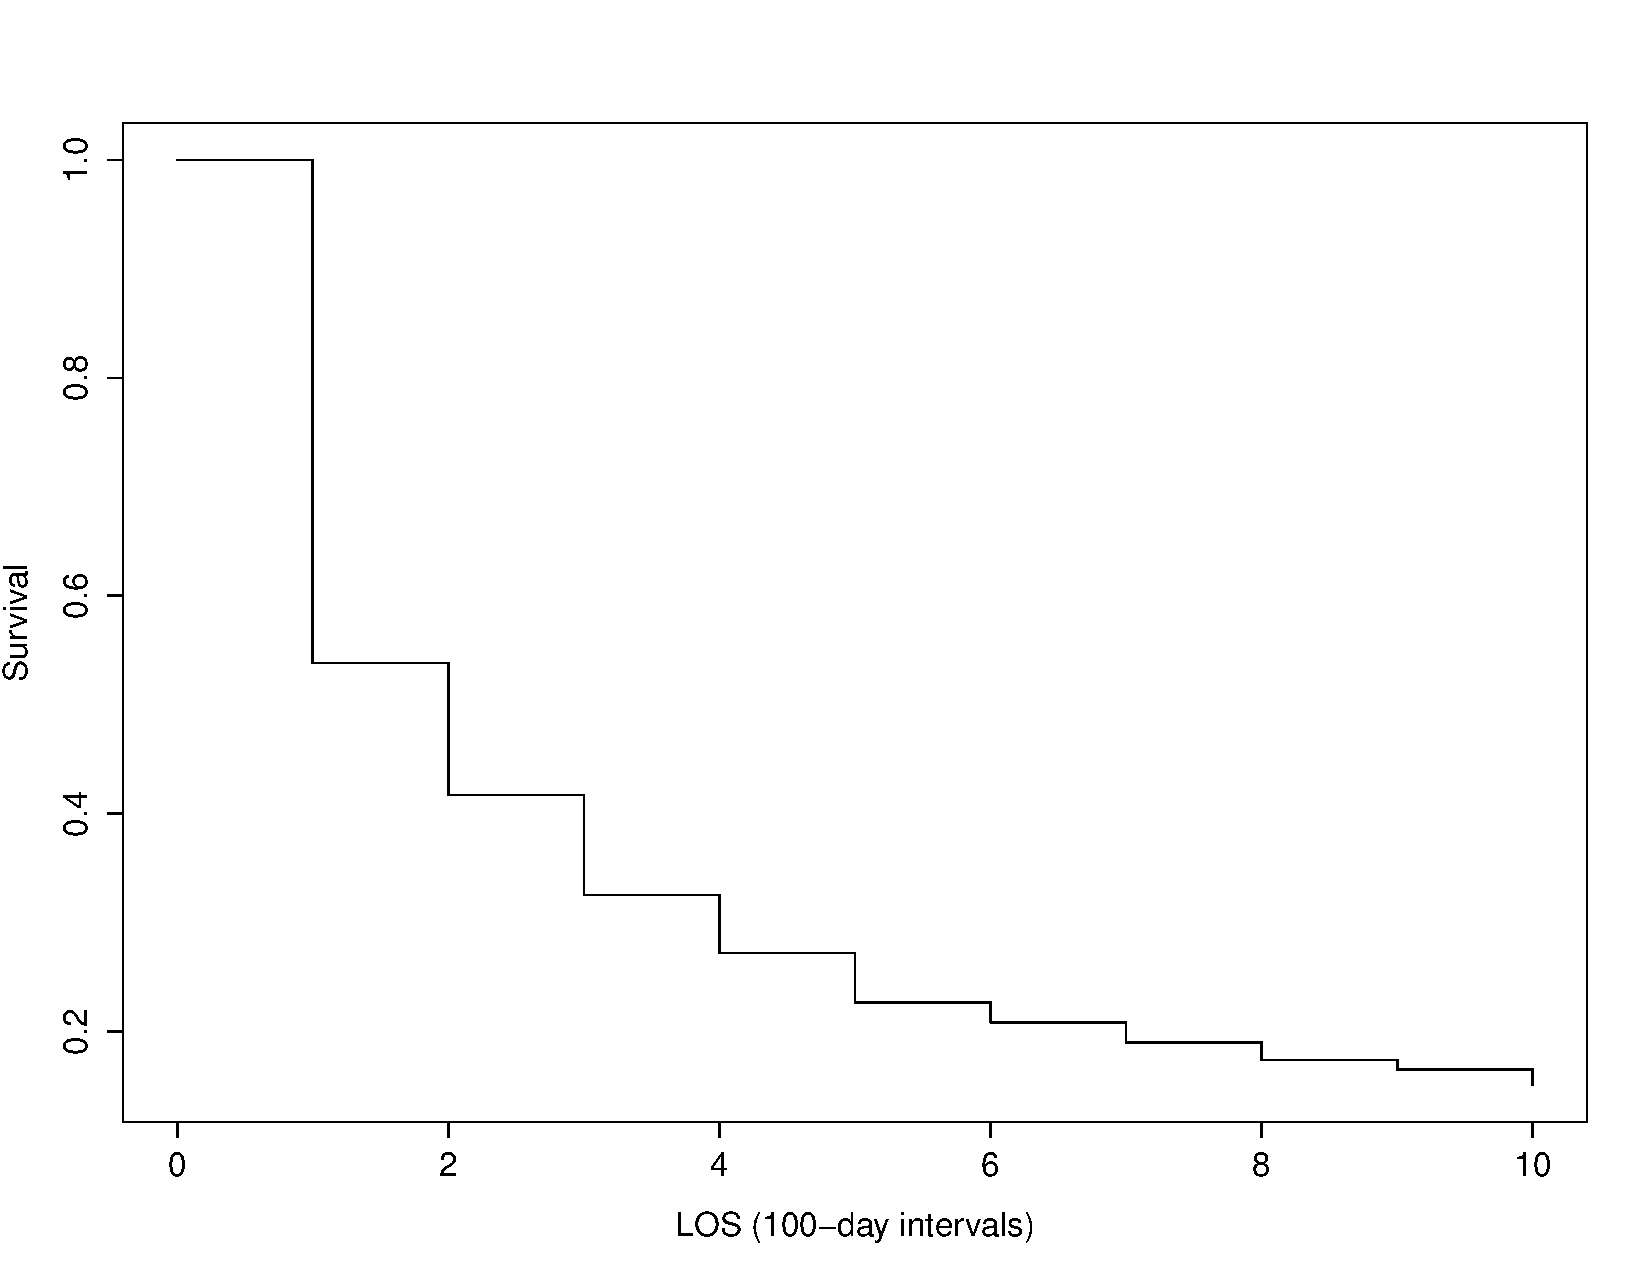
\includegraphics[width=4in]{nhact_surv.pdf}}
\caption{\bf Estimated Survival}
\end{figure}
%\vspace*{-.05in}
\begin{figure}[h!]
\centerline{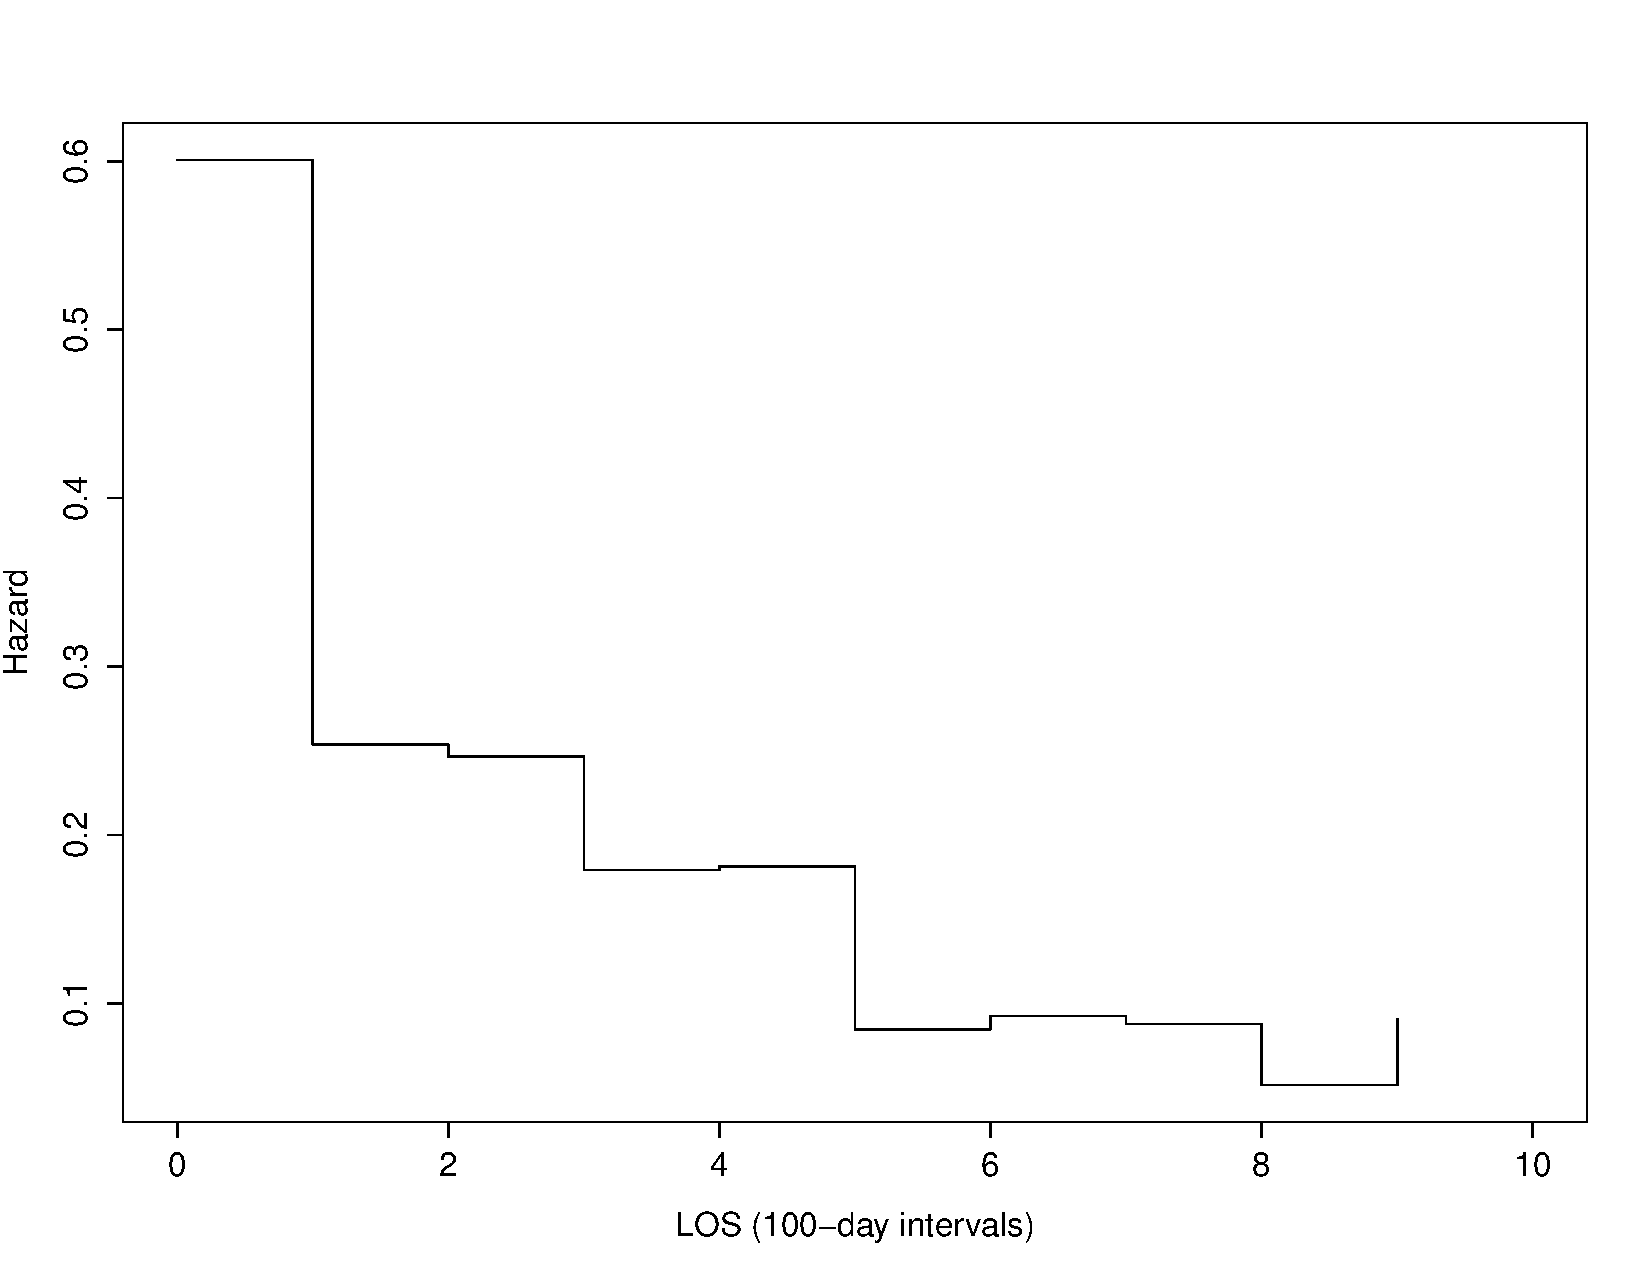
\includegraphics[width=4in]{nhact_haz.pdf}}
\caption{Estimated hazard}
\end{figure}
\newpage
\section{Estimating the cumulative hazard; the Nelson-Aalen estimator}
Suppose we want to estimate $\Lambda(t) = \int_{0}^{t} \lambda(u) du$, the
cumulative hazard at time t.

Just as we did for the KM, think of dividing the observed
timespan of the study into a series of fine intervals so
that there is only one event per interval: \\[2ex]
\begin{center}
\begin{tabular}{l|p{.2in}|p{.2in}|p{.2in}
|p{.2in}|p{.2in}|p{.2in}|p{.2in}|p{.2in}|p{.2in}|p{.2in}
|p{.2in}|p{.2in}|p{.2in}}
&   &  & D & & C & & C & D & D & D \\ \hline
\end{tabular}
\end{center}
%\vspace*{.5in}
$\Lambda(t)$ can then be approximated by a sum:
\[  \hat{\Lambda}(t) = \sum_{j}  \lambda_j  \Delta \]
where the sum is over intervals, $\lambda_j$ is the
value of the hazard in the $j$-th interval and
$\Delta$ is the width of each  interval.  Since $\hat{\lambda} \Delta$
is approximately the probability of dying in the interval, we
can further approximate by
   \[  \hat{\Lambda}(t) = \sum_{j}  d_j/r_j \]\\
It follows that $\Lambda(t)$ will change only at death times,
and hence we write the Nelson-Aalen estimator as:
   \[  \hat{\Lambda}_{\small NA}(t) = \sum_{j: \tau_j<t}  d_j/r_j \]
%%%%%%%%%%%%%%%%%%%%%%%%%%%%%%%%%%%%%%%%%%%%%%%%%%%%
\section{The Fleming-Harrington (FH) estimator}
\begin{center}
\begin{tabular}{l|p{.2in}|p{.2in}|p{.2in}
 |p{.2in}|p{.3in}|p{.2in}|p{.2in}|p{.2in}|p{.2in}|p{.2in}
 |p{0.2in}|p{.2in}|p{.2in}|}
  &   &  & D & & C & & C &  D & D & D \\ \hline
$r_j$ &  n & n & n & n-1 & n-1& n-2 & n-2 & n-3 & n-4  & \\
$d_j$ &  0 & 0 & 1 & 0   & 0  & 0   & 0   & 1   & 1   & \\
$c_j$ &  0 & 0 & 0 & 0   & 1  & 0   & 1   & 0   & 0   &  \\[2ex]
$\hat{\lambda}(t_j)$ & 0 & 0 & 1/n &  0  &  0  & 0   &  0
& $\frac{1}{n-3}$ &  $\frac{1}{n-4}$  & \\[2ex]
$\hat{\Lambda}(t_j)$ & 0 & 0 & 1/n & 1/n & 1/n & 1/n & 1/n & & &  \\
\end{tabular}
\end{center}
Once we have $\hat{\Lambda}_{\tiny NA}(t)$, we can also find another estimator
of $S(t)$ (Fleming-Harrington):
     \[  \hat{S}_{\tiny FH}(t) = \exp(-\hat{\Lambda}_{\tiny NA}(t)) \]
In general, this estimator of the survival function will be close to
the Kaplan-Meier estimator, $\hat{S}_{\tiny KM}(t)$
We can also go the other way ... we can take the Kaplan-Meier estimate
of $S(t)$, and use it to calculate an alternative estimate of the
cumulative hazard function:
\begin{eqnarray*}
\hat\Lambda_{\tiny KM}(t) & = & - \log \hat{S}_{\tiny KM}(t)
\end{eqnarray*}
\end{document}
%%%%%%%%%%%%%%%%%%%%%%%%%%%%%%%%%%%%%%%%%%%%%%%%%%%%
\subsection{Stata commands for FH Survival Estimate}

Say we want to obtain the Fleming-Harrington estimate of the survival
function for married females, in the healthiest initial subgroup,
who are randomized to the untreated group of the nursing home study.
\\[2ex]
First, we use the following commands to calculate the Nelson-Aalen
cumulative hazard estimator:
\begin{verbatim}
. use nurshome

. keep if rx==0 & gender==0 & health==2 & married==1
 (1579 observations deleted)

. sts list, na
         failure _d:  fail
   analysis time _t:  los

           Beg.          Net   Nelson-Aalen    Std.
  Time    Total   Fail   Lost    Cum. Haz.    Error   [95% Conf. Int.]
----------------------------------------------------------------------
    14       12      1      0      0.0833    0.0833   0.0117    0.5916
    24       11      1      0      0.1742    0.1233   0.0435    0.6976
    25       10      1      0      0.2742    0.1588   0.0882    0.8530
    38        9      1      0      0.3854    0.1938   0.1438    1.0326
    64        8      1      0      0.5104    0.2306   0.2105    1.2374
    89        7      1      0      0.6532    0.2713   0.2894    1.4742
   113        6      1      0      0.8199    0.3184   0.3830    1.7551
   123        5      1      0      1.0199    0.3760   0.4952    2.1006
   149        4      1      0      1.2699    0.4515   0.6326    2.5493
   168        3      1      0      1.6032    0.5612   0.8073    3.1840
   185        2      1      0      2.1032    0.7516   1.0439    4.2373
   234        1      1      0      3.1032    1.2510   1.4082    6.8384
----------------------------------------------------------------------
\end{verbatim}
\normalsize
After generating the Nelson-Aalen estimator, we manually
have to create a variable for the survival estimate:
\begin{verbatim}
. sts gen nelson=na
. gen sfh=exp(-nelson)
. list sfh

           sfh
  1.  .9200444
  2.  .8400932
  3.  .7601478
  4.  .6802101
  5.  .6002833
  6.  .5203723
  7.  .4404857
  8.  .3606392
  9.  .2808661
 10.  .2012493
 11.  .1220639
 12.  .0449048

\end{verbatim}
Additional built-in functions can be used to generate 95\%
confidence intervals on the FH survival estimate (to be covered
in lab session).
\\[2ex]
We can compare the Fleming-Harrington survival estimate to the KM
estimate by rerunning the {\tt sts list} command:
\begin{verbatim}

. sts list

. sts gen skm=s

. list skm sfh

            skm        sfh
  1.  .91666667   .9200444
  2.  .83333333   .8400932
  3.        .75   .7601478
  4.  .66666667   .6802101
  5.  .58333333   .6002833
  6.         .5   .5203723
  7.  .41666667   .4404857
  8.  .33333333   .3606392
  9.        .25   .2808661
 10.  .16666667   .2012493
 11.  .08333333   .1220639
 12.          0   .0449048

\end{verbatim}
In this example, it looks like the Fleming-Harrington estimator is
slightly higher than the KM at every time point, but with larger
datasets the two will typically be much closer.
\end{document}
